\documentclass{article}
\usepackage[utf8]{inputenc}
\usepackage[T1]{fontenc}
\usepackage{xcolor}
\usepackage{amsmath}
\usepackage{tikz}
\usetikzlibrary{positioning, shapes, arrows.meta, fit, backgrounds}

\newcommand{\featT}[3]{\texttt{tc#1[#2]@#3}}

\begin{document}

        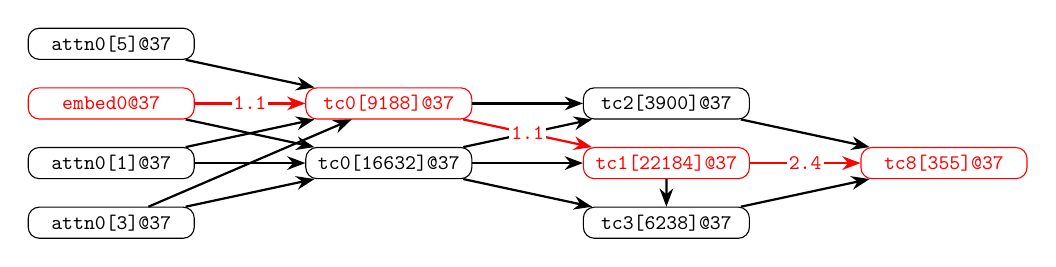
\begin{tikzpicture}[
    node distance=1em and 4em, %
    mynode/.style={
        draw, 
        minimum height=1.5em, 
        minimum width=8em, 
        font=\ttfamily, 
        scale=.75, 
        rounded corners
    },
    arrow/.style={-Stealth, thick},
    labelnode/.style={
        fill=white, 
        inner sep=1pt, 
        font=\ttfamily,
        scale=.75
    },
]

\node[mynode] (r1c1) {attn0[5]@37};
\node[mynode, below=of r1c1, color=red] (r1c2) {embed0@37};
\node[mynode, below=of r1c2] (r1c3) {attn0[1]@37};
\node[mynode, below=of r1c3] (r1c4) {attn0[3]@37};

\node[mynode, right=of r1c2, color=red] (r2c2) {\featT{0}{9188}{37}};
\node[mynode, right=of r1c3] (r2c3) {\featT{0}{16632}{37}};

\draw[arrow] (r1c1) -- (r2c2);
\draw[arrow] (r1c2) -- (r2c3);
\draw[arrow] (r1c3) -- (r2c2);
\draw[arrow] (r1c3) -- (r2c3);
\draw[arrow] (r1c4) -- (r2c2);
\draw[arrow] (r1c4) -- (r2c3);
\draw[arrow, color=red] (r1c2) -- (r2c2) node[midway, labelnode] {1.1};

\node[mynode, right=of r2c2] (r3c2) {\featT{2}{3900}{37}};
\node[mynode, right=of r2c3, color=red] (r3c3) {\featT{1}{22184}{37}};

\draw[arrow] (r2c2) -- (r3c2);
\draw[arrow] (r2c3) -- (r3c2);
\draw[arrow] (r2c3) -- (r3c3);
\draw[arrow, color=red] (r2c2) -- (r3c3) node[midway, labelnode] {1.1};

\node[mynode, below=of r3c3] (r4c4) {\featT{3}{6238}{37}};

\draw[arrow] (r2c3) -- (r4c4);
\draw[arrow] (r3c3) -- (r4c4);

\node[mynode, right=of r3c3, color=red] (r5c2) {\featT{8}{355}{37}};

\draw[arrow] (r3c2) -- (r5c2);
\draw[arrow] (r4c4) -- (r5c2);
\draw[arrow, color=red] (r3c3) -- (r5c2) node[midway, labelnode] {2.4};
\end{tikzpicture}

\end{document}